%%-*-latex-*-

\documentclass[compress,dvipdfmx]{beamer}

\usepackage[T1]{fontenc}
\usepackage[english]{babel}
\usepackage{amssymb,amsmath}
\usepackage{xspace}

% Draws a bounding line box frame:
%\usepackage[center, frame, axes]{crop}

% Language
%
\usepackage{hyphenat}          % \hyp{} is a breakable dash
\usepackage{alltt}
\usepackage{beramono}          % Bold in verbatim

\frenchspacing  % Follow French conventions after a period

% Maths & Logic
%
\usepackage{stmaryrd}
\usepackage{mathpartir}

% Graphics
%
\usepackage{graphicx}

% New environments and commands
%

% Input files
%
\newcommand\Inria{\textbf{Inria}\xspace}
\newcommand\Tezos{\textbf{Tezos}\xspace}
\newcommand\Nomadic{\emph{Nomadic Labs (Paris)}\xspace}
\newcommand\FV[1]{\mathcal{F}({#1})}
% Typesetting
%
\newcommand\mypar[1]{\paragraph{#1}\addcontentsline{toc}{subsection}{#1}}
%\newenvironment{sverb}{\small\verbatim}{\endverbatim}
\newenvironment{sverb}{\verbatim}{\endverbatim}

% The TeXbook, Exercise 11.6, p. 311.
%
\def\myfrac#1/#2{\leavevmode\kern.1em
\raise.5ex\hbox{\the\scriptfont0 #1}\kern-.1em
/\kern-.15em\lower.25ex\hbox{\the\scriptfont0 #2}}

% Terms and rules
%
\newcommand\ttcons[2]{{#1}\,$::$\,{#2}}
\newcommand\cons[2]{{#1}\!::\!{#2}}
\newcommand\el{[\,]}
\newcommand\fun[1]{\textsf{#1}}
\newcommand\xkwd[1]{\textsf{\textbf{#1}}}
\newcommand\ufun[1]{\underline{\fun{#1}}}
\newcommand\Lla[1]{\Lleftarrow_{\!{\smash{#1}}}}
\newcommand\Rra[1]{\Rrightarrow_{\!{\smash{#1}}}}

% Languages
%
\newcommand\Coq{\textsf{Rocq}\xspace}
\newcommand\Blang{\textsf{B~language}\xspace}
\newcommand\Simulink{\textsf{Simulink}\xspace}
\newcommand\Lustre{\textsf{Lustre}\xspace}
\newcommand\Esterel{\textsf{Esterel}\xspace}
\newcommand\Promela{\textsf{Promela}\xspace}
\newcommand\UPPAAL{\textsf{UPPAAL}\xspace}
\newcommand\SPIN{\textsf{SPIN}\xspace}
\newcommand\Saxon{\textsf{Saxon}\xspace}
\newcommand\Unicode{\textsf{Unicode}\xspace}
\newcommand\MIME{\textsf{MIME}\xspace}
\newcommand\XML{\textsf{XML}\xspace}
\newcommand\XMLSchema{\textsf{XML Schema}\xspace}
\newcommand\XSLT{\textsf{XSLT}\xspace}
\newcommand\XQuery{\textsf{XQuery}\xspace}
\newcommand\HTML{\textsf{HTML}\xspace}
\newcommand\XHTML{\textsf{XHTML}\xspace}
\newcommand\HTTP{\textsf{HTTP}\xspace}
\newcommand\DTD{\textsf{DTD}\xspace}
\newcommand\Scheme{\textsf{Scheme}\xspace}
\newcommand\XPath{\textsf{XPath}\xspace}
\newcommand\Erlang{\textsf{Erlang}\xspace}
\newcommand\Haskell{\textsf{Haskell}\xspace}
\newcommand\Clean{\textsf{Clean}\xspace}
\newcommand\Prolog{\textsf{Prolog}\xspace}
\newcommand\Java{\textsf{Java}\xspace}
\newcommand\OCaml{\textsf{OCaml}\xspace}
\newcommand{\CamlpF}{\textsf{Camlp4}\xspace}
\newcommand\ocamllex{\textsf{ocamllex}\xspace}
\newcommand\menhir{\textsf{menhir}\xspace}
\newcommand\ocamlyacc{\textsf{ocamlyacc}\xspace}
\newcommand\Ada{\textsf{Ada}\xspace}
\newcommand\Clang{\textsf{C}\xspace}
\newcommand\Michelson{\textsf{Michelson}\xspace}
\newcommand\Fstar{\textsf{F}\(^{*}\)\xspace}
\newcommand\Fsharp{\textsf{F}\(^\sharp\)\xspace}
\newcommand\HACLstar{\textsf{HACL}\(^{*}\)\xspace}
\newcommand\Unix{\textsf{Unix}\xspace}
\newcommand\Cpp{\mbox{\textsf{C} \hspace*{-1.5mm} \raise 0.7mm \hbox
{${\scriptscriptstyle \textsf{++}}$}}\xspace}

% Figures
%
\newcommand\fig{\textsc{figure}}
\newcommand\Fig{\textsc{Figure}}
\newcommand\figs{\textsc{figures}}

% Costs
%
\newcommand\Cost{\mathcal{C}}
\newcommand\Best{\mathcal{B}}
\newcommand\Worst{\mathcal{W}}
\newcommand\Mean{\mathcal{A}}
\newcommand\Trace{\mathcal{T}}
\newcommand\Seq{\mathcal{S}}

\newcommand\C[2]{\Cost_{#2}^{#1}}
\newcommand\B[2]{\Best_{#2}^{#1}}
\newcommand\W[2]{\Worst_{#2}^{#1}}
\newcommand\M[2]{\Mean_{#2}^{#1}}
\newcommand\T[2]{\Trace_{#2}^{#1}}
\newcommand\Call[1]{\Cost\llbracket{#1}\rrbracket}
\newcommand\A[1]{\Seq_{#1}}

\newcommand\Expected[1]{\mathbb{E}[{#1}]}

\newcommand\OC[2]{\OCost_{#2}^{\raisebox{-2.5pt}{$\scriptstyle #1$}}}
\newcommand\OB[2]{\OBest_{#2}^{\raisebox{-2.5pt}{$\scriptstyle #1$}}}
\newcommand\OW[2]{\OWorst_{#2}^{\raisebox{-2.5pt}{$\scriptstyle #1$}}}
\newcommand\OM[2]{\OMean_{#2}^{\raisebox{-2.5pt}{$\scriptstyle #1$}}}
\newcommand\OT[2]{\OTrace_{#2}^{\raisebox{-2.5pt}{$\scriptstyle #1$}}}

\newcommand\OCost{\overline{\Cost}}
\newcommand\OBest{\overline{\Best}}
\newcommand\OWorst{\overline{\Worst}}
\newcommand\OMean{\overline{\Mean}}

% Number-theoretic functions
%
\newcommand\floor[1]{\lfloor{#1}\rfloor}
\newcommand\ceiling[1]{\lceil{#1}\rceil}

% Rewrite systems
%
\newcommand\len[1]{\lvert{#1}\rvert{}}
\newcommand\eqn[1]{\mathrel{\stackrel{\smash{#1}}{=}}}
\newcommand\pair[2]{\langle{#1},{#2}\rangle}
\newcommand\measure[1]{\mathcal{M}\llbracket{#1}\rrbracket}

% Induction
%
\newcommand\total{\succ^t}
\newcommand\predName[1]{\textsf{#1}}
%\newcommand\pred[2]{\predName{#1}\llparenthesis{#2}\rrparenthesis}
\newcommand\pred[2]{\predName{#1}({#2})}

% Word Factoring
%
\newcommand\wlen[1]{\lVert{#1}\rVert{}}
\newcommand\ind[2]{{#1}[{#2}]}
\newcommand\Ind[2]{\ind{#1}{#2}}
\newcommand\BorderName{\mathfrak{B}}
\newcommand\Border[2]{\BorderName^{#1}(#2)}
\newcommand\DBorder[3]{\BorderName_{#1}^{#2}(#3)}
\newcommand\MPfailureName{\mathfrak{F}}
\newcommand\MPfailure[3]{\MPfailureName_{#1}^{#2}(#3)}

\newcommand\prefeqSym{\trianglelefteqslant}    % Prefix
\newcommand\nprefeqSym{\ntrianglelefteqslant}
\newcommand\prefSym{\triangleleft}
\newcommand\nprefSym{\ntriangleleft}

\newcommand\prefeq{\mathrel{\prefeqSym}}
\newcommand\nprefeq{\mathrel{\nprefeqSym}}
\newcommand\pref{\mathrel{\prefSym}}
\newcommand\npref{\mathrel{\nprefSym}}

\newcommand\prefeqName{\mathord{\prefeqSym}}
\newcommand\nprefeqName{\mathord{\nprefeqSym}}
\newcommand\prefName{\mathord{\prefSym}}
\newcommand\nprefName{\mathord{\nprefSym}}

\newcommand\word[1]{\fun{#1}}

% Java keywords
%
\newcommand\abstractX{\texttt{\textbf{abstract}}}
\newcommand\class{\texttt{\textbf{class}}}
\newcommand\extends{\texttt{\textbf{extends}}}
\newcommand\final{\texttt{\textbf{final}}}
\newcommand\main{\texttt{\textbf{main}}}
\newcommand\new{\texttt{\textbf{new}}}
\newcommand\protectedX{\texttt{\textbf{protected}}}
\newcommand\private{\texttt{\textbf{private}}}
\newcommand\public{\texttt{\textbf{public}}}
\newcommand\return{\texttt{\textbf{return}}}
\newcommand\static{\texttt{\textbf{static}}}
\newcommand\super{\texttt{\textbf{super}}}
\newcommand\this{\texttt{\textbf{this}}}
\newcommand\void{\texttt{\textbf{void}}}
\newcommand\nullX{\texttt{\textbf{null}}}
\newcommand\booleanX{\texttt{\textbf{boolean}}}
\newcommand\ifX{\texttt{\textbf{if}}}
\newcommand\elseX{\texttt{\textbf{else}}}
\newcommand\throw{\texttt{\textbf{throw}}}
\newcommand\throws{\texttt{\textbf{throws}}}

% Typesetting Erlang
%
\newcommand\erlcode[1]{\texttt{#1}}
\newcommand\clause[1]{\(#1\)}
\newcommand\smashedrightarrow[1]{\xrightarrow{\smash{#1}}}
\newcommand\smashedleftarrow[1]{\xleftarrow{\smash{#1}}}
\newcommand\MyArrow[2]{\smashedrightarrow{\makebox[#1][c]{\(_\mathrm{#2}\)}}}
\newcommand\fbcode[1]{{\setlength\fboxsep{0mm}\fbox{\phantom{\(\raisebox{-1pt}{#1}\)}}}}
\newcommand\obp{\textbf{(}}
\newcommand\cbp{\textbf{)}}

%% Queues (requires stmaryrd)
%
\newcommand\enq[2]{#1 \mathbin{\Yleft} #2}
\newcommand\deq[2]{#2 \mathbin{\Yright} #1}
\newcommand\emq{\mathord{\circleddash}}

%% Grammars
%
\newcommand\first[1]{\mathcal{P}(#1)}
\newcommand\follow[1]{\mathcal{S}(#1)}

% Beamer configuration
%
\usetheme{default}
\setbeamersize{text margin left=6mm}
\setbeamersize{text margin right=6mm}
\setbeamertemplate{headline}{}
\setbeamertemplate{navigation symbols}{}
\setbeamertemplate{footline}[page number]{}
\setbeamertemplate{itemize items}[circle]
\setbeamertemplate{theorems}[numbered]


% ----------------------------------------------------------------
% Document
%
\title{Formal Methods in Software Engineering}
\author{Christian Rinderknecht}
\institute{Eszterházy Károly Katolikus Egyetem}
\date{September 2026}

\begin{document}

\frame{\maketitle}

\begin{frame}
  \frametitle{Introduction}

  This lecture is meant to present what \textbf{formal methods} are,
  in particular in the context of \textbf{software engineering}.

  \bigskip

  It provides you with the industrial context and theoretical
  framework within which you can proceed to practical knowledge.

  \bigskip

  I will teach you a bit of \OCaml, as functional languages are a good
  framework to illustrate some proofs of programs.

\end{frame}


\begin{frame}
  \frametitle{Complex software is everywhere... and has bugs}

  \begin{center}
    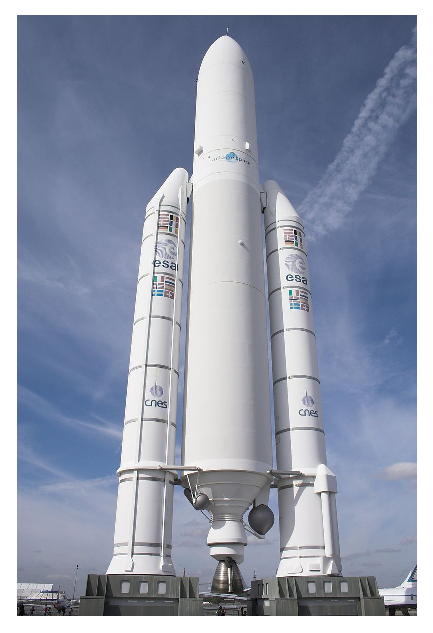
\includegraphics[scale=0.6]{Ariane_5.eps}
  \end{center}

  \centerline{Ariane 5. Credit: ignis, GFDL, CC BY-SA-2.5,2.0,1.0.}

\end{frame}


\begin{frame}
  \frametitle{The case of Ariane~5}

  In June 1996, the maiden launch of the European rocket Ariane~5
  ended in its self\hyp{}destruction.

  \bigskip

  The cause was in the software controlling the trajectory.

  \bigskip

  This piece of software was designed with the requirements of
  Ariane~4, \textbf{not} Ariane~5.

  \bigskip

  Accordingly, some ranges of physical parameters were taken from
  Ariane~4, and wrongly assumed in the programming of Ariane~5.

  \bigskip

  Therefore, certain errors were deemed impossible for physical
  reasons and not handled in the code.

  \bigskip

  During the flight, a value overflowed, causing an exception to be
  raised, but not handled, which lead to the self\hyp{}destruction of
  the launcher (the control system believed that the rocket was
  off\hyp{}course).

\end{frame}


\begin{frame}
  \frametitle{The case of Ariane~5}

  The language used to program that piece of software in Ariane~5 was
  \Ada.

  \bigskip

  \Ada is a programming language originally designed in France in the
  early 80s, before it became the official language for most
  developments for the defence of the USA.

  \bigskip

  \Ada is used a lot in critical embedded systems, deployed in
  transport, aerospace and defence.

  \bigskip

  The language was carefully designed so it lends itself well to all
  sorts of \textbf{static analyses}.

  \bigskip

  These analyses are static because they are performed by the \Ada
  compiler itself, or by other tools that read the source code.

  \bigskip

  Their aim can vary, but perhaps the most important is \textbf{the
    detection of run\hyp{}time errors} before the code is deployed.

\end{frame}


\begin{frame}
  \frametitle{The case of Ariane~5 / The after...math}

  The catastrophic failure of the first Ariane~5 incurred a very high
  cost, and the loss of ten years of research and development in
  satellite technology.

  \bigskip

  \Ada itself is not to blame.

  \bigskip

  Instead of going into the details of what went wrong, let us
  consider what happened next.

  \bigskip

  Some researchers at \Inria (Gonthier \& Deutsch) proposed a static
  analyser for \Ada that could have caught the error that lead to the
  loss of Ariane~5, and discovered many other errors.

  \bigskip

  The mathematical theory they used to analyse the software is called
  \textbf{abstract interpretation}.

  \bigskip

  This powerful theory was invented in the 70s by the French
  researchers Patrick and Radhia Cousot.

\end{frame}


\begin{frame}
  \frametitle{PolySpace Technologies}

  In 1999, a start-up company called \textbf{PolySpace Technologies}
  was founded in France by Alain Deutsch (\Inria) and Daniel Pilaud
  (co\hyp{}inventor of \Lustre, a declarative language for programming
  synchronous systems).

  \bigskip

  I joined that company in 2000 to work on the static analysis of
  JavaCard. The idea was to translate JavaCard and other languages
  (\Clang and \Cpp) to \Ada, for which there was already a static
  analyser, following the explosion of Ariane~5.

  \bigskip

  The translation did not need to preserve all behaviours, only those
  who could go wrong (run\hyp{}time errors).

  \bigskip

  The company was a success and is now part of \textbf{Mathworks
    Inc.}, known for MATLAB and \Simulink.

  \bigskip

  PolySpace (the tool) is well known in the avionics industry.

\end{frame}


\begin{frame}
  \frametitle{Abstract interpretation}

  \textbf{Abstract interpretation} is a general framework to analyse
  programs and systems.

  \bigskip

  It makes an \textbf{over\hyp{}approximation} of the behaviours of a
  program, then deduce properties on those, and finally translates
  back the abstract properties in terms of the original behaviours of
  the program.

  \bigskip

  Abstract interpretation is used to replace a system with a possibly
  infinite or very large number of states with a system that has a
  small number of states that can all be checked exhaustively.

  \bigskip

  Abstract interpretation can also be used to \textbf{prove the
    absence of errors}, or to find errors.

\end{frame}


\begin{frame}
  \frametitle{Abstract interpretation / An illustration}

  As an illustration, let us consider a system whose states are pairs
  of positive natural numbers, represented as coordinates on a quarter
  of plane.

  \bigskip

  A \textbf{state} is all the information characterising a system
  running at a given point in time (memory contents, program counter,
  files, network buffers, etc.)

  \bigskip

  Some states are coloured in \textcolor{red}{red} to denote that they
  are erroneous: this is the property `To be erroneous'.

  \bigskip

  A behaviour of a system, or \textbf{trace}, can be thought as a line
  from one state to the next. We show four traces as black, thick
  lines.

  \bigskip

  One of the traces actually ends in an error.

\end{frame}


\begin{frame}
  \frametitle{Abstract interpretation / An illustration}

  \vspace*{15mm}
  \includegraphics[bb=95 428 500 727, scale=0.7]{traces}

\end{frame}


\begin{frame}
  \frametitle{Abstract interpretation / An illustration}

  We need to characterise the erroneous states in a simple manner, at
  the cost of over\hyp{}approximating them: this means to abstract the
  property `To be erroneous' so it becomes easier to check.

  \bigskip

  For example, we can abstract the error property by a red square
  containing the set of erroneous states, instead of being the set
  itself.

  \bigskip

  A square can be defined by three numbers only, and it is easy to
  check whether a given state belongs to it: if so, we deem it an
  error.

  \bigskip

  In our example, this creates \textbf{false positives}, that is,
  states inside the square that are not actual errors.

\end{frame}


\begin{frame}
  \frametitle{Abstract interpretation / An illustration}

  \vspace*{15mm}
  \includegraphics[bb=95 428 500 727, scale=0.7]{traces}

\end{frame}

\begin{frame}
  \frametitle{Abstract interpretation / An illustration}

  \vspace*{15mm}
  \includegraphics[bb=95 428 500 727, scale=0.7]{traces_square}

\end{frame}

\begin{frame}
  \frametitle{Abstract interpretation / An illustration}

  \vspace*{15mm}
  \includegraphics[bb=95 428 500 727, scale=0.7]{traces_square_cropped}

\end{frame}

\begin{frame}
  \frametitle{Abstract interpretation / An illustration}

  To reduce the number of false positives, we \textbf{refine the
    abstract property} so it fits better the erroneous states.

  \bigskip

  For instance, we could use another polygon to cover more tightly the
  erroneous states.

  \bigskip

  Let us try an hexagon: to define it, we need the same amount of
  information as for a square, but the inclusion property is slightly
  more complex.

  \bigskip

  This is better, but one trace remains a false positive. In general,
  false positives are inevitable if the property is complex enough, so
  trade\hyp{}offs are necessary.

\end{frame}


\begin{frame}
  \frametitle{Abstract interpretation}

  \vspace*{15mm}
  \includegraphics[bb=85 428 500 727, scale=0.7]{traces_square_cropped}

\end{frame}


\begin{frame}
  \frametitle{Abstract interpretation}

  \vspace*{15mm}
  \includegraphics[bb=85 428 500 727, scale=0.7]{traces_hexagon}

\end{frame}


\begin{frame}
  \frametitle{A success story: the Parisian métro line~14}

  \begin{center}
    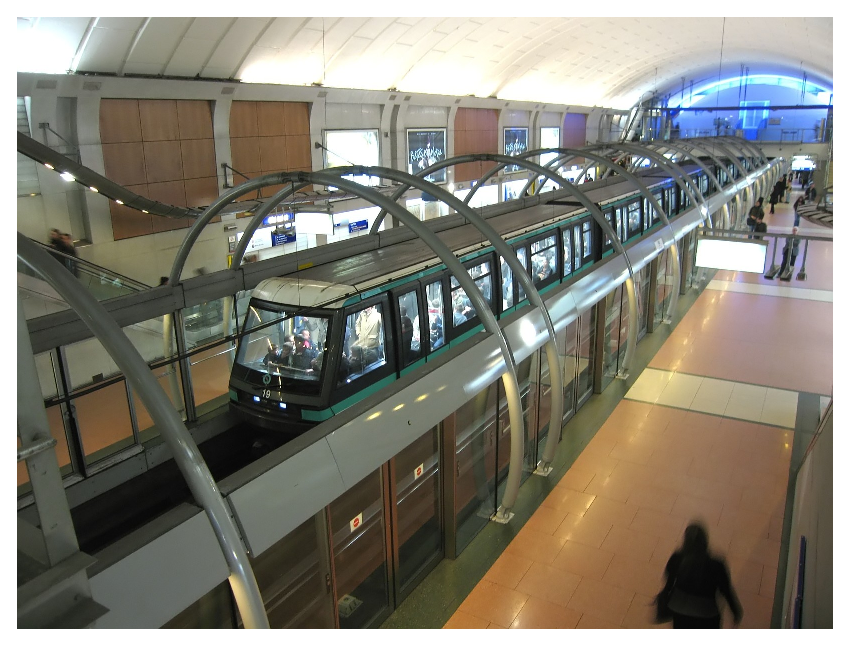
\includegraphics[scale=0.6]{ligne-14-Chatelet.eps}
  \end{center}

  \centerline{M\'etro line~14. Credit: Pline, CC BY-SA-3.0}

\end{frame}


\begin{frame}
  \frametitle{The Parisian métro line~14}

  In October 1999, opened in Paris the first entirely automated metro
  line (number~14).

  \bigskip

  Some people thought that the trains were controlled at a distance,
  but they actually moved and stopped based on decisions taken by
  themselves, with inputs from sensors and communication networks.

  \bigskip

  To ensure such a high\hyp{}level of safety and continuity of
  service, the company Matra Transport used formal methods from the
  start of the project.

  \bigskip

  After the success of that new metro line, an existing metro line
  (number~1) has been automatised successfully.

  \bigskip

  \textbf{Railways signalling systems} are a major user of formal
  methods, due to the high safety requirements.

\end{frame}


\begin{frame}
  \frametitle{The Parisian métro line~14}

  The train system comprises four subsystems:
  \begin{enumerate}
    \item the automatic pilot and signalling system,

    \item the operation control centre,

    \item the platform doors,

    \item the audio-video system.
  \end{enumerate}

  \bigskip

  Only the first  subsystem includes software that is  critical to the
  safety of the passengers.

  \bigskip

  It controls the movement of trains (speed, traction power, routes)
  and the doors (on\hyp{}board and on the platforms).

  \bigskip

  It sends any alarm to the operation control centre.

\end{frame}


\begin{frame}
  \frametitle{The Parisian métro line~14}

  The system architecture is naturally distributed and is made of
  \begin{enumerate}

    \item the line equipment, in the operation control centre,

    \item the wayside equipment along the tracks,

    \item the on\hyp{}board equipment.

  \end{enumerate}

  \bigskip

  They are interlinked via a high\hyp{}speed communication network.

\end{frame}


\begin{frame}
  \frametitle{The Parisian métro line~14}

  In the operation control centre, operators monitor scheduled train
  programs for each day and supervise events received from the
  network.

  \bigskip

  Platform doors prevent people from falling on the tracks. The train
  doors open only when they are aligned with the platform doors.

  \bigskip

  If not properly aligned, there are emergency doors on the platform
  that can be manually opened.

  \bigskip

  Audio and video feeds allows operators to monitor the inside the
  carriages and to speak with passengers (a high\hyp{}level of
  availability is required to ensure security).

\end{frame}


\begin{frame}
  \frametitle{The Parisian métro line~14}

  In order to bring strong correctness assurances in software, it is
  paramount to carefully specify the expected behaviours and delimit
  the field of application of the mathematical proofs.

  \bigskip

  The use of the \textbf{B~method} by Matra Transport International
  (now part of Siemens) for the Parisian metro line~14 is a case in
  point of this approach. (Another example is the Calcutta metro, in
  1992.)

  \bigskip

   The B~method was invented in the 80s by Jean-Raymond Abrial, a
   French researcher. It comprises
   \begin{enumerate}

     \item a formal notation to expression specifications,

     \item a design methodology,

     \item and software tools as a support.

   \end{enumerate}

\end{frame}


\begin{frame}
  \frametitle{The B~method}

  The formal \textbf{\Blang} is based on \textbf{set theory}, which
  makes it very expressive. It enables the specification of a system
  and its expected properties into a model called an \textbf{abstract
    machine}.

  \bigskip

  It also enables the proof of such properties (like safety): some as
  \textbf{system invariants} (properties that must hold on all
  states), some as \textbf{postconditions} to mathematical functions.

  \bigskip

  A \textbf{proof assistant} then either automatically proves some of
  these theorems, or requests the engineer to prove them
  interactively.

  \bigskip

  The B~method and its software tools allow the engineer to
  \textbf{refine} the abstract machine into a series of abstract
  machines until a \textbf{concrete machine} is obtained. A concrete
  machine is one that can be translated automatically into a
  programming language (\Clang or \Ada).

\end{frame}


\begin{frame}
  \frametitle{The B~method}

  Each abstract machine is, in turn, less and less
  \textbf{denotational}, and more and more \textbf{operational}.

  \bigskip

   `Operational' means `what a system does', whereas `denotational'
  means `what properties the system satisfies'.

  \bigskip

  Step by step, the abstract machines become closer to
  \textbf{algorithms}, that is, functions operating over data
  structures, which is what a concrete machine is about.

  \bigskip

  The other aspect of a concrete machine is that it is
  \textbf{deterministic}: there are no unspecified choices left in the
  control flow (`what to do next' is always explicit).

\end{frame}


\begin{frame}
  \frametitle{The B~method / Refinement}

  \begin{center}
    \includegraphics[bb=71 519 505 721, scale=0.75]{refinement}
  \end{center}

\end{frame}


\begin{frame}
  \frametitle{The B~language / An abstract machine}

  An abstract machine in the B~language consists of
  \begin{itemize}

    \item \textbf{states}, that is, variables satisfying some
      invariant properties, and

    \item \textbf{operations}, that is, functions that change the
      state while maintaining the invariants, and return values.

  \end{itemize}

  \bigskip

  The variables making up the state of an abstract machine can denote
  mathematical sets, relations, functions, etc.

  \bigskip

  Operations are defined with
  \begin{itemize}

    \item \textbf{preconditions}: `What is assumed about the state by
      the operation before starting', and

    \item \textbf{postconditions}: `What can be assumed about the
      state and return value after the operation is finished'.

  \end{itemize}

\end{frame}


\begin{frame}
  \frametitle{The B~language / An abstract machine}

  Let us specify in the B~language what is the Greatest Common Divisor
  (GCD) of two natural numbers.

  \bigskip

  In English: `The GCD of \(x\)~and~\(y\) is~\(d\) such that \(d\)
  divides both \(x\)~and~\(y\), and any divisor of~\(x\) and~\(y\) is
  lower than or equal to~\(d\).'

  \bigskip

  In mathematical notation:
  \begin{equation*}
    \tiny
    \gcd(x,y) \mid x \quad\land\quad
    \gcd(x,y) \mid y \quad\wedge\quad
    \forall z.(z \mid x \;\;\wedge\;\; z \mid y
    \;\; \Rightarrow\;\; z \leqslant \gcd(x,y)).
  \end{equation*}

  The next slide shows the equivalent definition in the B~language
  (note that variables must be at least two characters long).

\end{frame}


\begin{frame}[fragile]
  \frametitle{Greatest Common Divisor (abstract)}

\begin{alltt}
\small
\textbf{MACHINE} gcd /* Greatest Common Divisor */
\textbf{OPERATIONS}
  rr <-- gcd (xx,yy) =
    \textbf{BEGIN}
      \textbf{PRE} xx : INT \& 1 <= xx \& xx < MAXINT
          yy : INT \& 1 <= yy \& yy < MAXINT
      \textbf{THEN}
        \textbf{ANY} dd \textbf{WHERE}
         dd : INT
            \& (xx-(xx/dd)*dd = 0) \& (yy-(yy/dd)*dd = 0)
            \& !zz.(zz : INT \& zz < MAXINT
                   \& (xx-(xx/zz)*zz = 0)
                   \& (yy-(yy/zz)*zz = 0) => zz <= dd)
        \textbf{THEN} rr := dd \textbf{END}
      \textbf{END}
    \textbf{END}
\end{alltt}

\end{frame}


\begin{frame}
  \frametitle{The B~method / Refinement}

  The refinement from the initial abstract machine to the final
  concrete machine is stepwise and the engineer must provide more
  details about the low\hyp{}level aspects of the system, whilst
  proving the new specification is \textbf{correct and complete} with
  respect to the previous one (all its behaviours are expected by the
  previous one, and vice\hyp{}versa).

  \bigskip

  This transitively entails that the concrete machine is
  \textbf{equivalent} to the initial abstract machine.

  \bigskip

  The last step consists in the \textbf{generation of \Ada programs}
  which are thus, by construction, correct and complete with respect
  to the initial specification.

\end{frame}


\begin{frame}[fragile]
  \frametitle{Greatest Common Divisor (concrete)}

\begin{alltt}
\small
\textbf{REFINEMENT} gcd_R1 /* refinement of ... */
\textbf{REFINES} gcd /* the previous machine */
\textbf{OPERATIONS}
 rr <-- gcd (xx,yy) = /* No room to handle xx < yy */
   \textbf{BEGIN}
     \textbf{PRE} xx : INT \& 1 <= xx \& xx < MAXINT
         yy : INT \& 1 <= yy \& yy < MAXINT
     \textbf{VAR} rem, old_xx, old_yy \textbf{IN}
     \textbf{WHILE} (yy != 0)
       old_xx := xold_yy := yyrem := xx-(xx/yy)*yy;
       xx := old_yyyy := rem
     \textbf{INVARIANT} gcd (old_xx, old_yy) = gcd (old_yy, rem)
     \textbf{VARIANT} yy < old_yy /* Termination */
     rr := xx
   \textbf{END}
\end{alltt}

\end{frame}

\begin{frame}[fragile]
  \frametitle{The B~language / Ada}

  From the concrete machine, the following \Ada code fragment would be
  produced, were the tooling told to inline the values of the
  variables \texttt{rr}, \texttt{old\_xx} and \texttt{old\_yy}, which
  are only needed for logical reasons (to state the invariant and
  variant, and the final result), not computational ones.
\begin{alltt}
\small
\textbf{function} GCD (Xx, Yy : Integer) \textbf{return} Integer \textbf{is}
  Rem : Integer
  \textbf{while} Yy /= 0 \textbf{loop}
    Rem := Xx \textbf{mod} Yy
    Xx := Yy
    Yy := Rem
  \textbf{end loop}
  \textbf{return} Xx
\textbf{end} GCD
\end{alltt}

\end{frame}


\begin{frame}
  \frametitle{Introduction (resumed)}

  Formal methods are methods and tools for software development that
  are grounded in theoretical computer science (informatics).

  \bigskip

  Some expected benefits are:
  \begin{itemize}

    \item the reduction in maintenance costs (e.g., corrective
      maintenance),

    \item more robustness (by explicitly delineating the domain of
      validity) and, more generally,

    \item higher reliability and levels of confidence.

  \end{itemize}

  \bigskip

  Formal methods are often applied in the making of \textbf{critical
    embedded systems} to guarantee safety and security, whenever human
  lives or large investments depend upon their correctness and
  continuity of service.

\end{frame}


\begin{frame}
  \frametitle{Astr\'ee}

  \begin{center}
    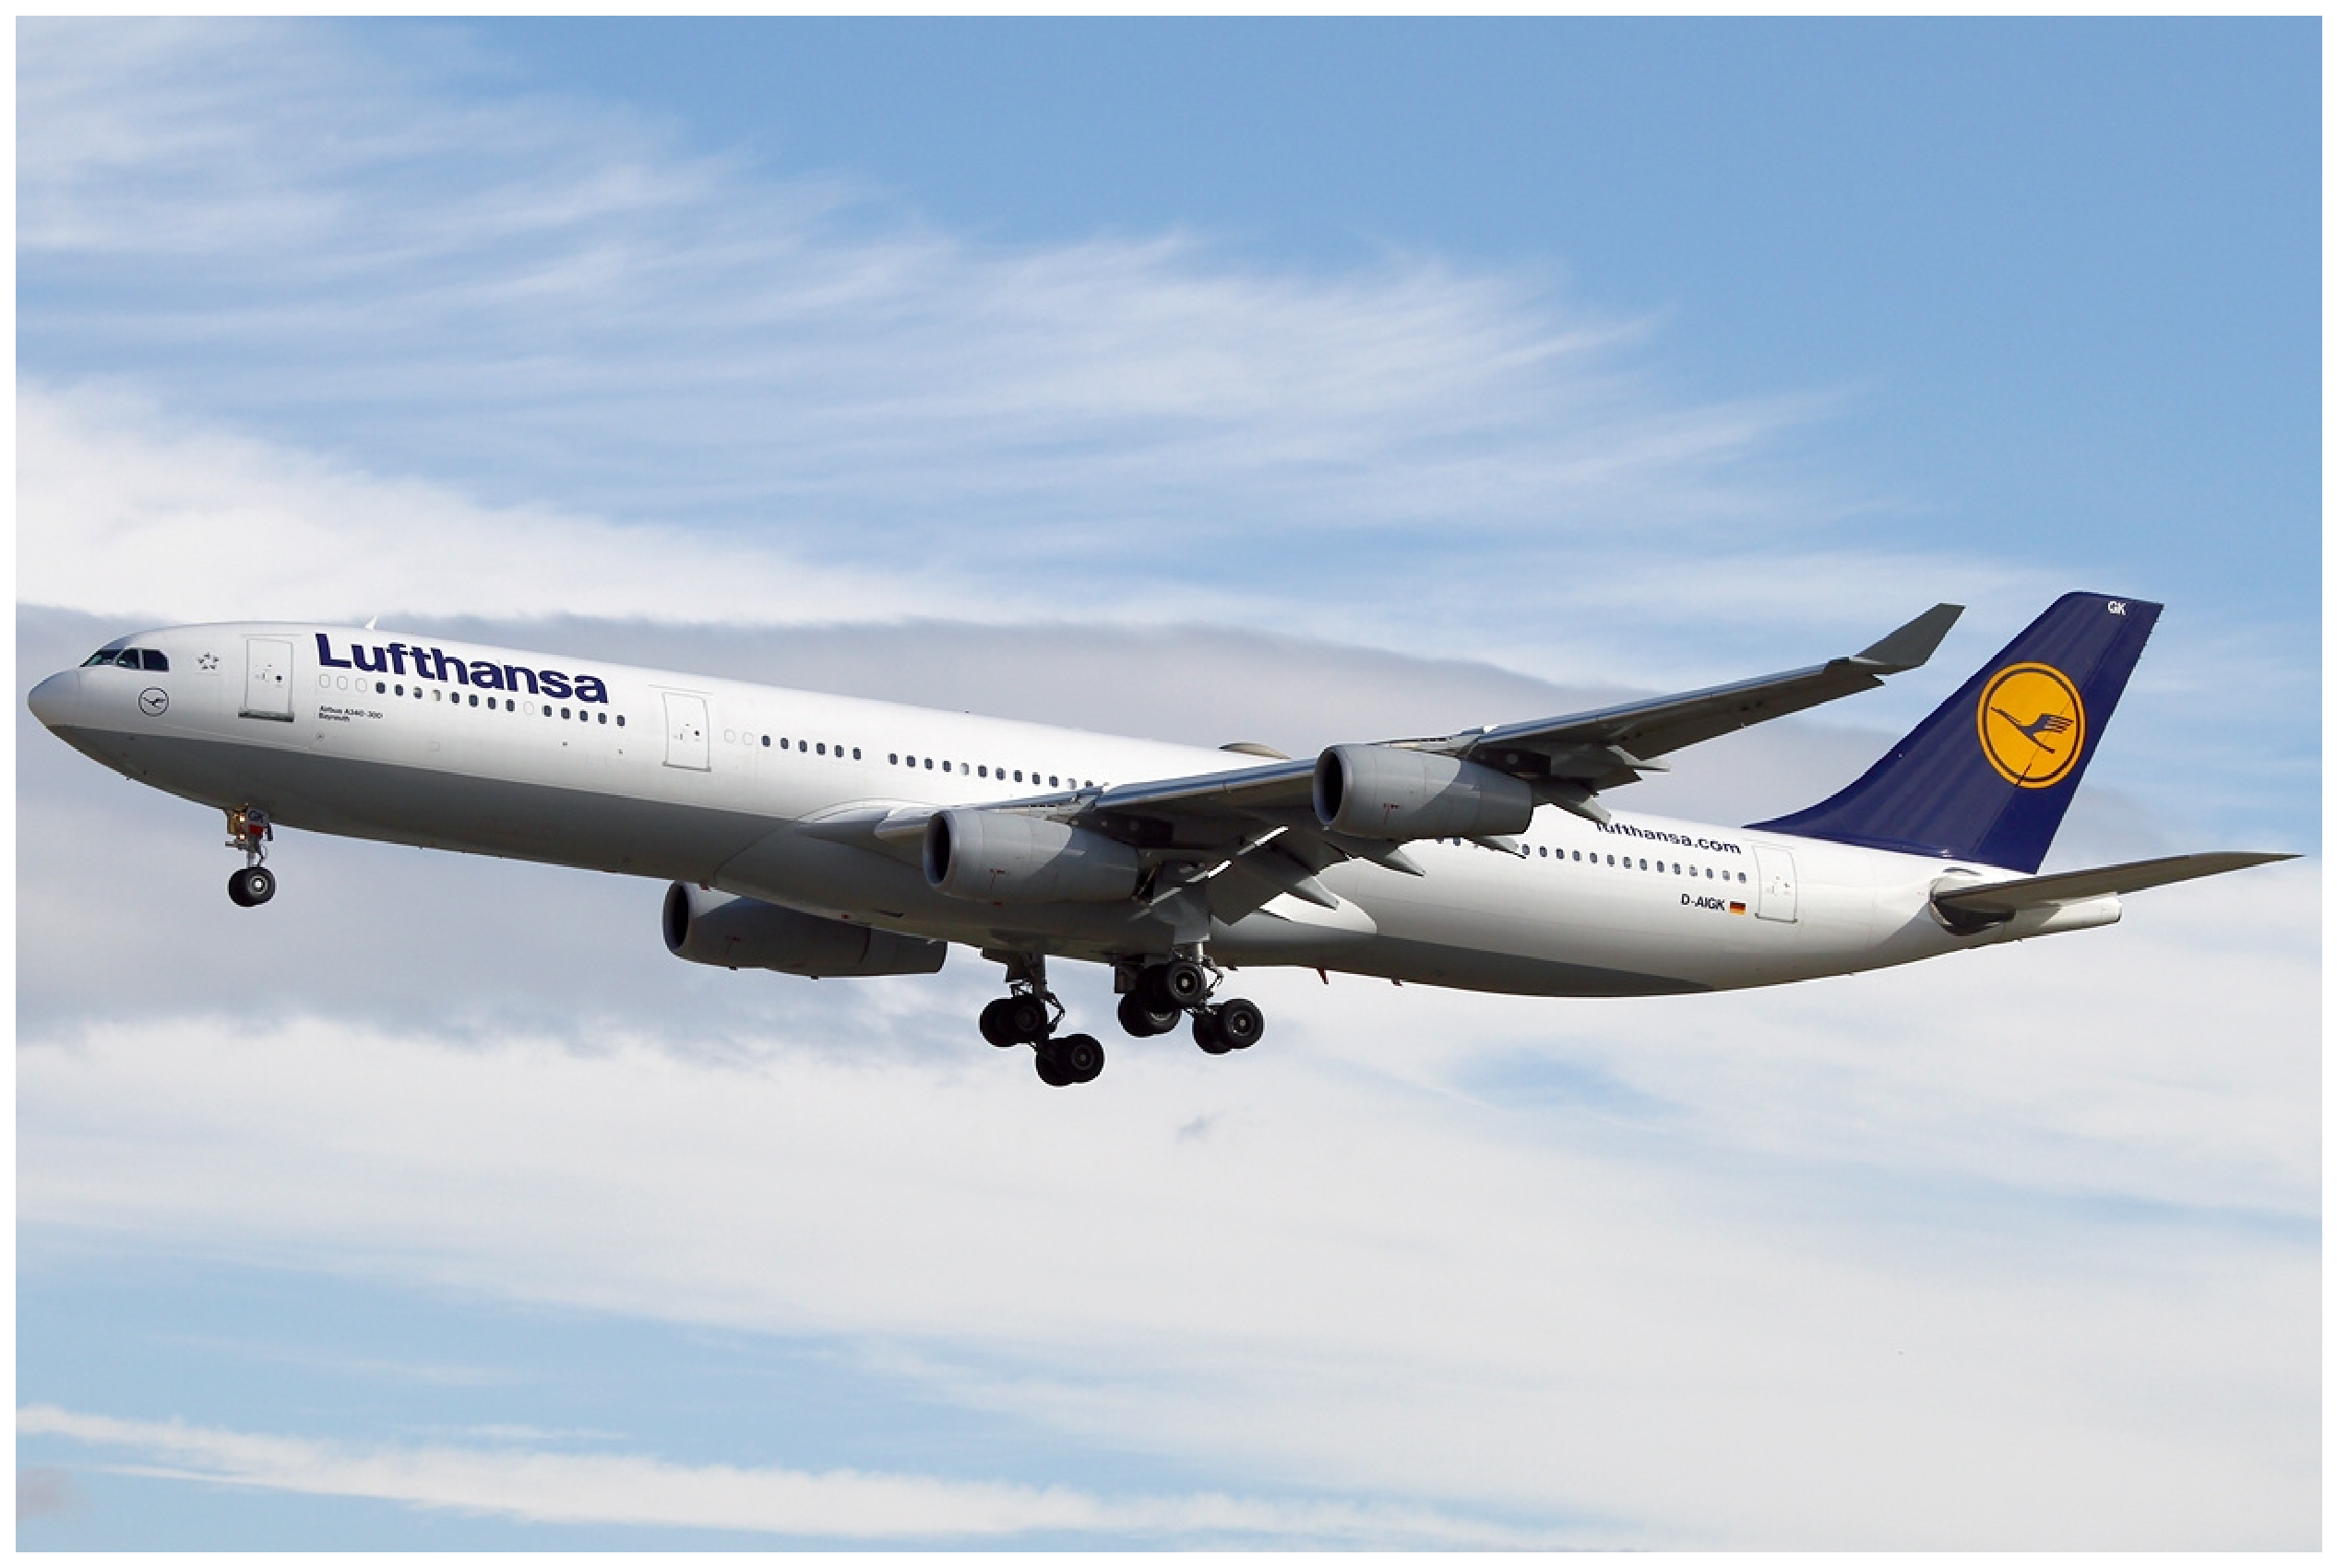
\includegraphics[scale=0.22]{Airbus_A340.eps}
  \end{center}

    \centerline{Airbus A340. Credit: Konstantin von Wedelstardt. GFDL
      1.2}

\end{frame}


\begin{frame}
  \frametitle{The static analyser Astr\'ee}

  The usefulness of formal methods should not be underestimated. They
  have taken decades to mature from academic research to practical
  frameworks, and are becoming more and more widespread.

  \bigskip

  Beyond PolySpace and the B~method, we can mention some other
  successful static analysers.

  \bigskip

  \textbf{Astr\'ee} offers an abstract interpretation of \Clang
  programs to detect run\hyp{}time errors, in the same vein as
  PolySpace. It was designed at \'Ecole Normale Sup\'erieure (France)
  and is now commercialised by the German company AbsInt.

  \bigskip

  In 2003, Astr\'ee proved automatically (on a standard PC) the
  absence of any run\hyp{}time errors in the primary flight control
  software of the Airbus A340 fly-by-wire system: 132,000 lines of
  \Clang. Astr\'ee is written in \OCaml and PolySpace in
  \textsf{Standard ML}, the American cousin of \OCaml.

\end{frame}


\begin{frame}
  \frametitle{The static analyser Frama-C}

  \begin{center}
    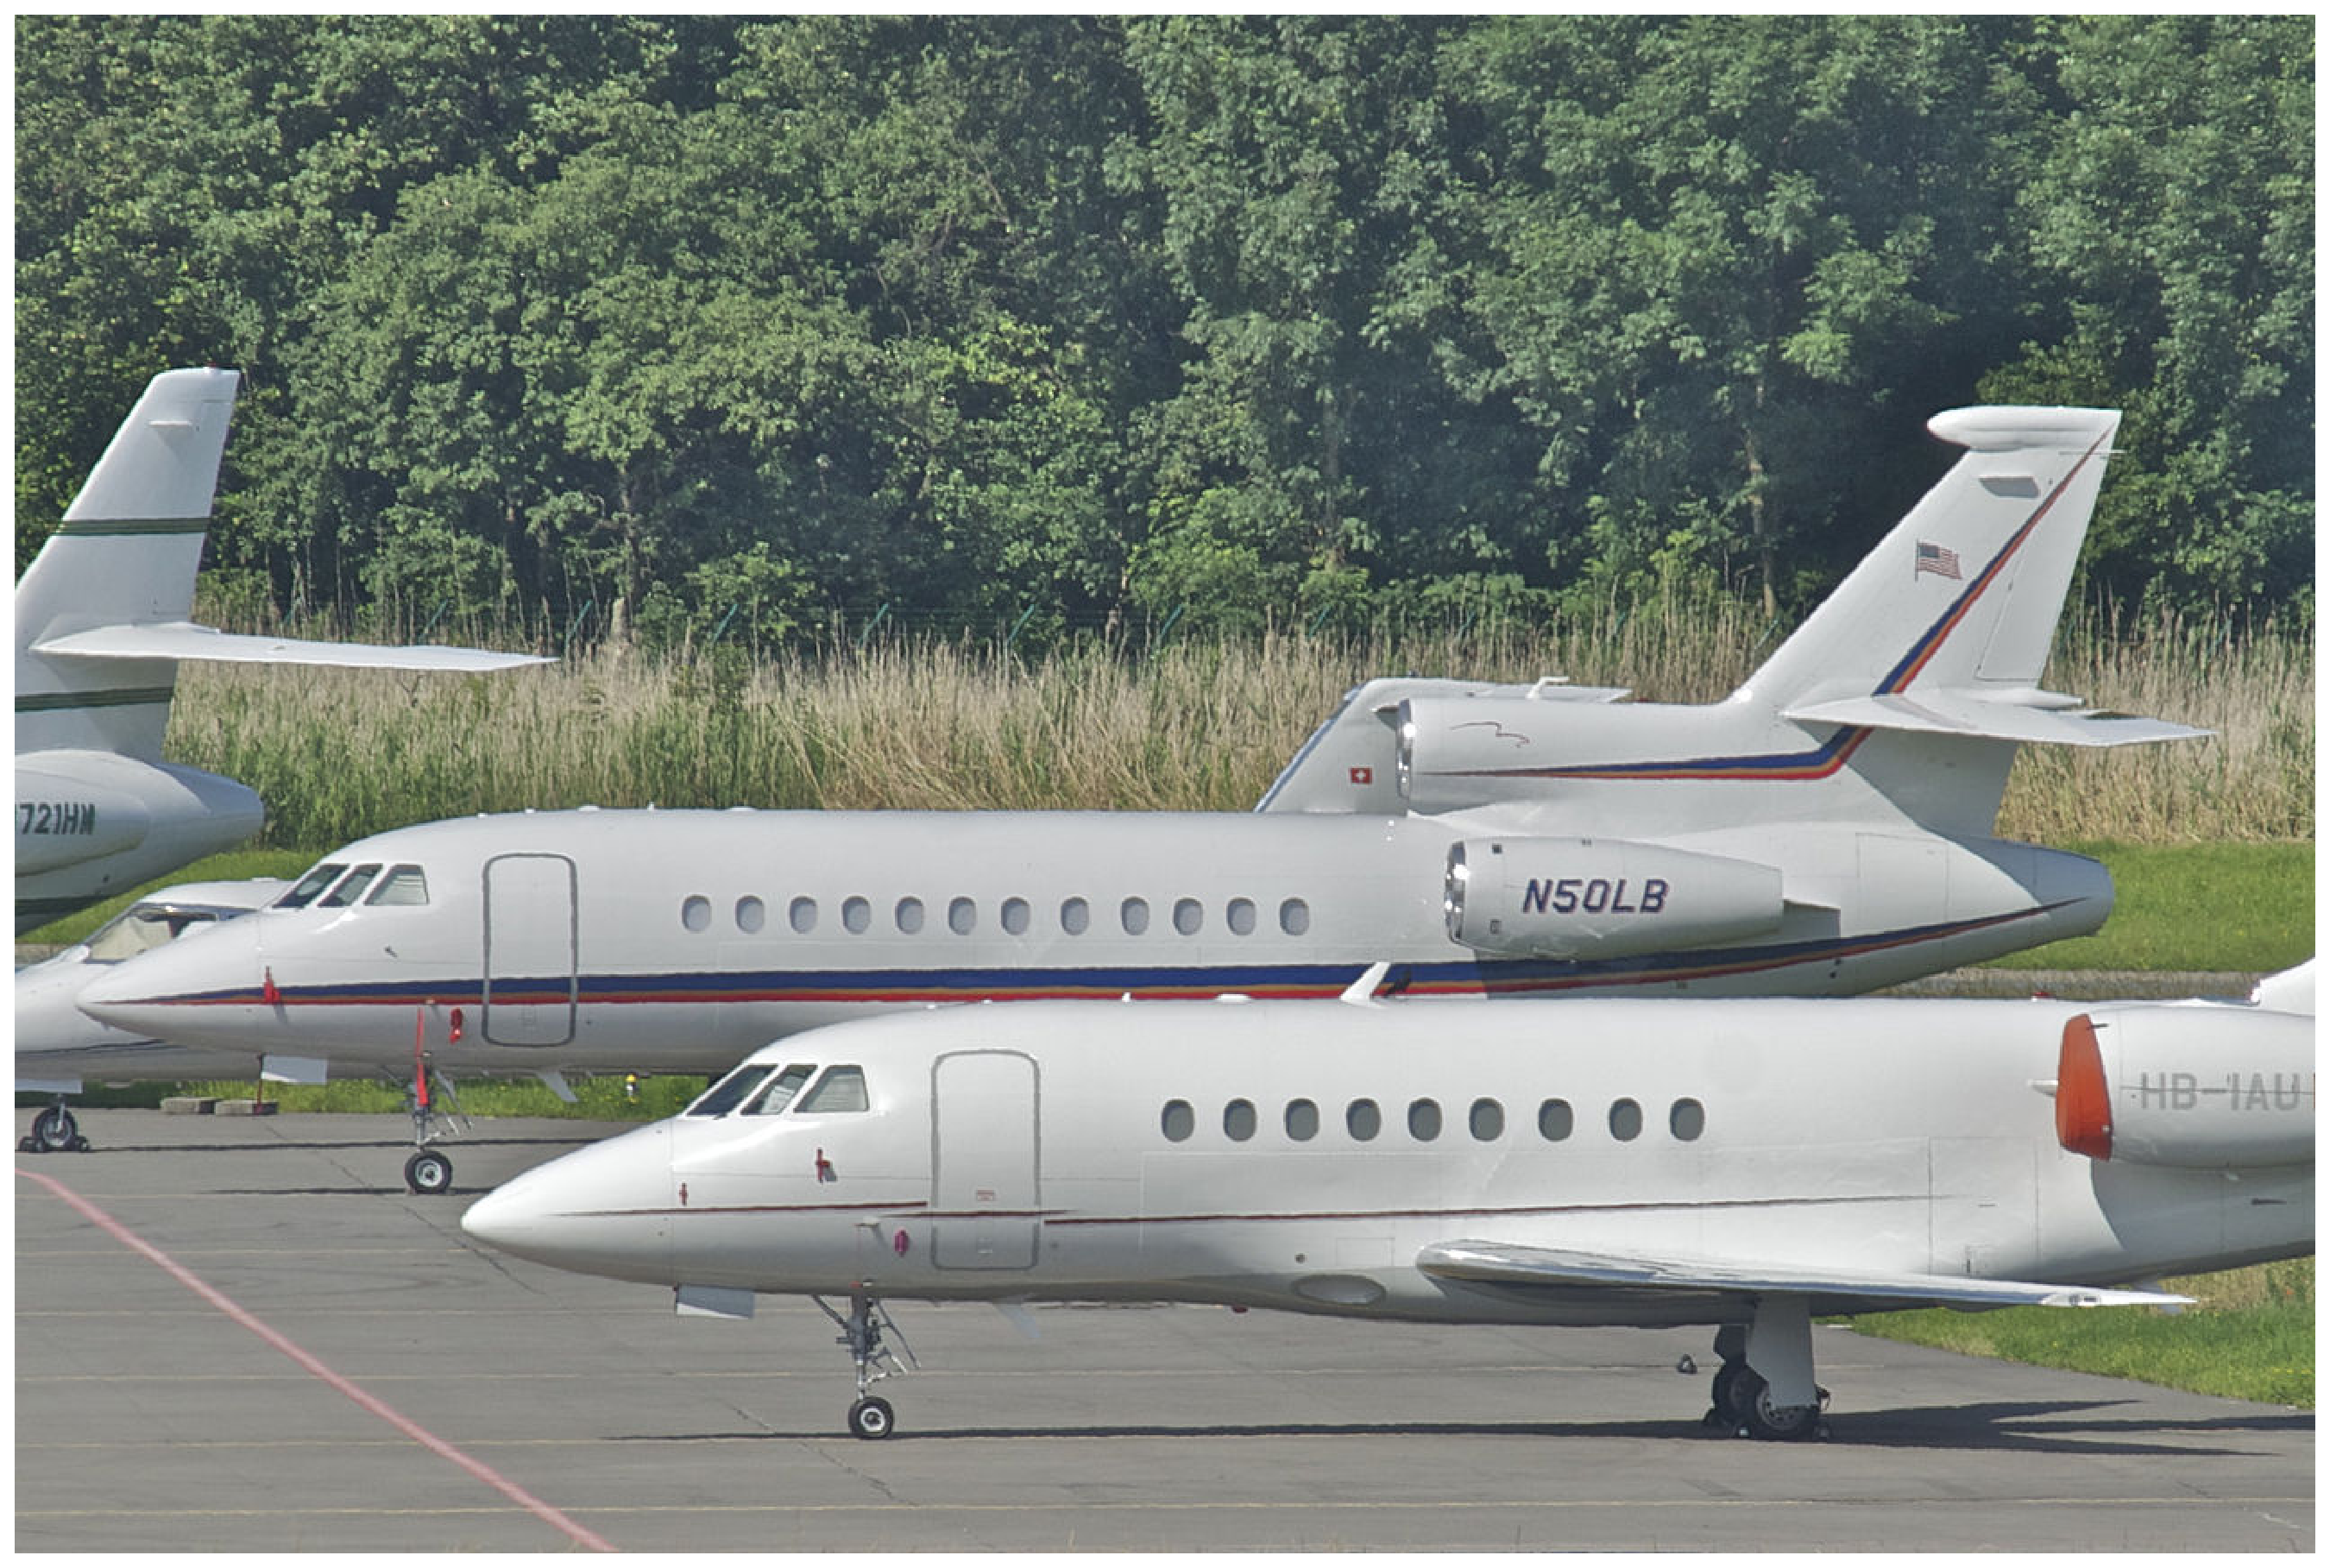
\includegraphics[scale=0.20]{Dassault_Falcon_900.eps}
  \end{center}

  \centerline{Dassault Falcon 900. Credit:  Aero Icarus, CC BY-SA-2.0}

\end{frame}


\begin{frame}
  \frametitle{The static analyser Frama-C}

  Another well\hyp{}known static analyser for \Clang is
  \textbf{Frama-C}. It was designed by researchers at the CEA
  (France).

  \bigskip

   Frama-C is actually a software suite which includes a static
   analyser, but also software to interactively prove that the source
   code satisfies some \textbf{functional specifications} provided by
   the user.

   \bigskip

   Recently, Frama-C has been used by Dassault Aviation to detect
   common weaknesses in real\hyp{}time software running on the Falcon
   jets.

   \bigskip The code base of Frama-C is almost entirely written in
   \OCaml (perhaps the largest \OCaml code base in the world).

\end{frame}


\begin{frame}
  \frametitle{Formal methods applied to compilers}

  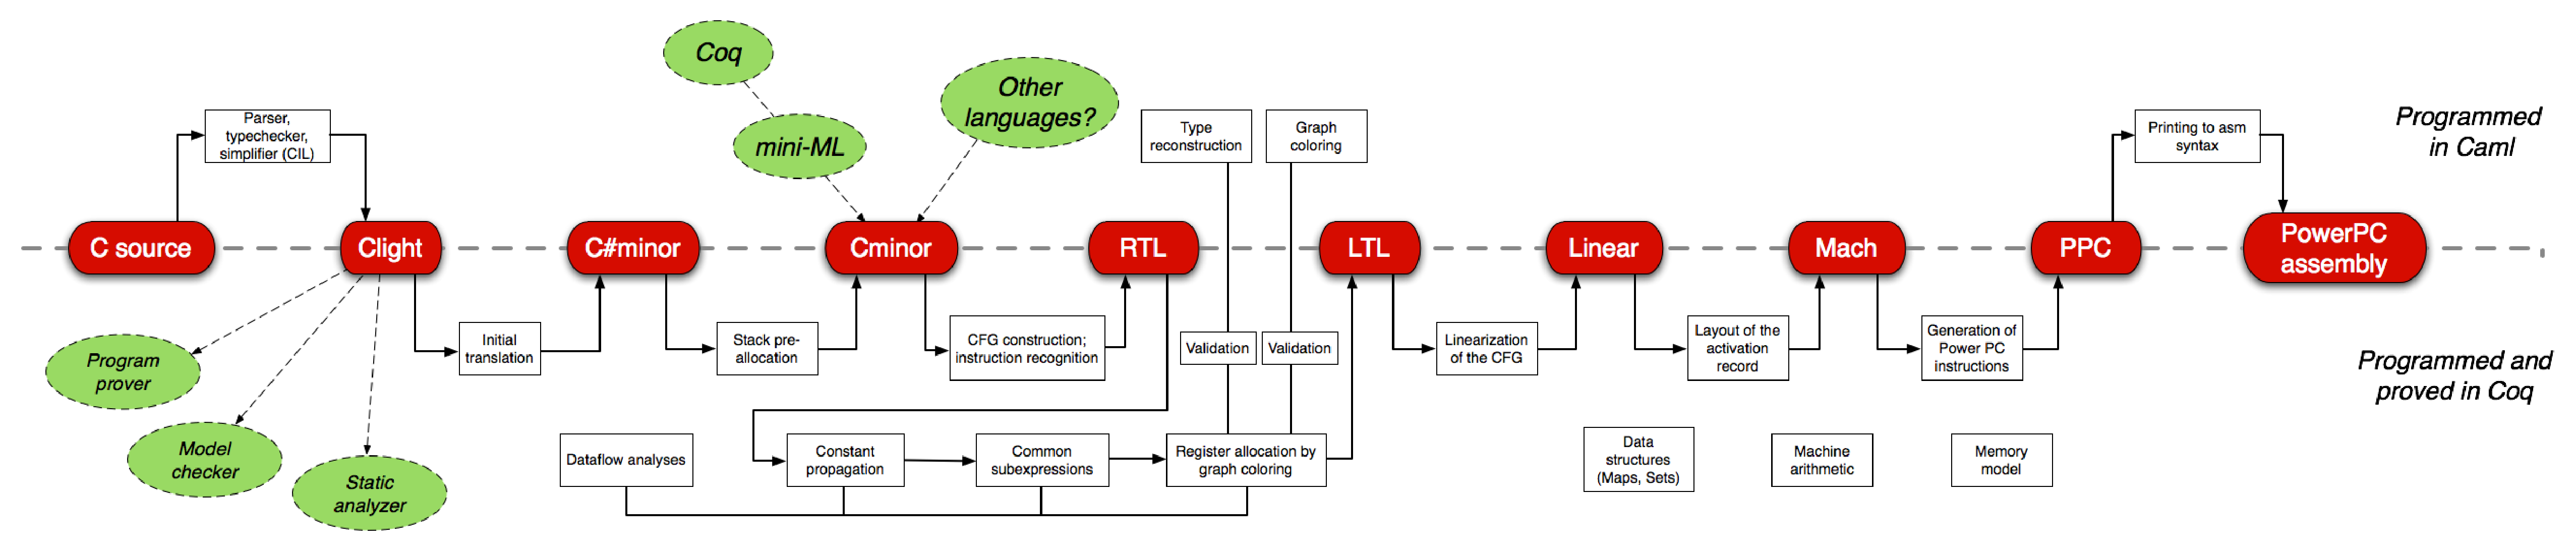
\includegraphics[scale=0.14,angle=35,origin=c]{CompCert_diagram.eps}

\end{frame}

\begin{frame}
  \frametitle{Formal methods applied to compilers}

  Formal methods can also be applied to \textbf{compilers}.

  \bigskip

  Compilers translate programs of high\hyp{}level languages (`close to
  human thought'), like \Clang, \Ada or \OCaml into programs of
  low\hyp{}level languages (`close to machine thought'), like assembly
  or byte\hyp{}code, and these two programs must be
  \textbf{operationally equivalent}.

  \bigskip

  This means that all behaviours of the input program must be
  preserved in the output program (\textbf{completeness}) and all
  behaviours of the output must map to behaviours of the input
  (\textbf{soundness}, also called \emph{correctness}).

  \bigskip

  Since \Clang is widespread in critical embedded software, it is
  desirable to consider \Clang compilers.

\end{frame}


\begin{frame}
  \frametitle{General architecture of a C compiler}

  The compiler is one link in a \textbf{tool chain}:

  \vspace*{-20mm}
  \includegraphics[bb=71 350 405 721,scale=0.55]{compilation_chain}

\end{frame}


\begin{frame}
  \frametitle{General architecture of a C compiler}

  There are two phases to compilation: \textbf{analysis} and
  \textbf{synthesis}.
  \begin{enumerate}

    \item The analysis breaks up the source program into
      constituent pieces of an intermediary representation of the
      program.

    \item The synthesis constructs the target program from this
      intermediary representation.

  \end{enumerate}

  \medskip

  Actually, there can be many intermediary representations, each one
  getting closer to the target language.

  \bigskip

  Each phase is itself decomposable into other phases, depending on
  the source and target languages.

\end{frame}


\begin{frame}
  \frametitle{General architecture of a C compiler}

  The first row makes up the analysis and the second is the synthesis.

  \smallskip

  \includegraphics[width=0.9\textwidth]{phases}

  A real compiler has many more stages than shown above, and is always
  a complex piece of software where more errors are likely. Those
  errors can be silent: some erroneous code can be emitted only for
  certain classes of programs, which is a serious problem for embedded
  applications.

  \bigskip

  Xavier Leroy at \Inria (France) has spearheaded the design and
  implementation of a \textbf{certified \Clang compiler}, called
  \textbf{CompCert}, using \Coq.

\end{frame}


\begin{frame}
  \frametitle{A formally verified C compiler: CompCert}

  CompCert is certified because its \textbf{\OCaml code has been
    extracted from the specification} (of a large subset) of \Clang
  and intermediary representations, as well as from
  \textbf{semantic\hyp{}preserving transformations} between those
  representations, down to optimised assembly.

  \bigskip

  John Regher and his colleagues are experts in finding bugs
  in \Clang compilers. They wrote, in 2011:
  \begin{quote}
    \textit{The striking thing about our CompCert results is that the
      middle\hyp{}end bugs we found in all other compilers are
      absent. [...] This is not for lack of trying: we have devoted
      about six CPU\hyp{}years to the task. The apparent
      unbreakability of CompCert supports a strong argument that
      developing compiler optimizations within a proof framework,
      where safety checks are explicit and machine-checked, has
      tangible benefits for compiler users.}
  \end{quote}

\end{frame}


\begin{frame}
  \frametitle{The proof assistant \Coq}

  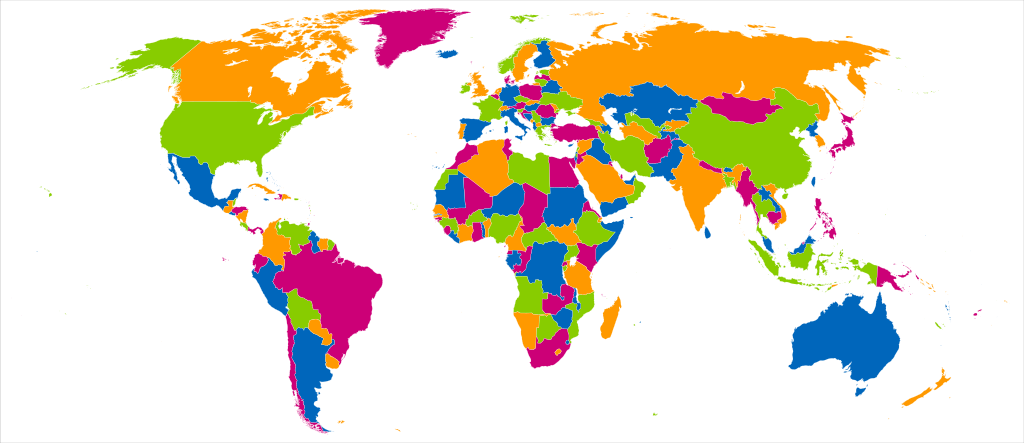
\includegraphics[scale=0.3]{world_map_with_four_colours.png}
  \centerline{Political map of the world. Credit: Fibonacci, CC BY-SA
    3.0}

\end{frame}


\begin{frame}
  \frametitle{The proof assistant \Coq}

  \begin{itemize}

    \item \Coq is a \textbf{proof assistant}, that is, a piece of
      software in which to express logical formulas, prove them and
      have the proofs checked automatically. It is an interactive
      tool, but it automates the search of some proof patterns
      (libraries called \textbf{tactics}).

    \item \Coq comes with a programming language named
      \textbf{Gallina} which is close to \OCaml, but \textbf{without
        side\hyp{}effects} and adding \textbf{dependent types}. This
      type system is more general than the type systems found in usual
      languages like \Java.

    \item \Coq features \textbf{code extraction}: it can generate an
      \OCaml program from the proof of its properties.

    %% \item A \textbf{constructive proof} is a proof in which for each
    %%   \(\exists\) quantifier, a witness is given: every object must be
    %%   explicitly built. In particular, this rules out the use of the
    %%   \textbf{law of excluded middle} of classical logic (\(\vdash A
    %%   \lor \neg A\)).

    \item Code extraction relies upon the \textbf{Curry\hyp{}Howard
      correspondence}, which states that a proof is analogous to a
      function, and the proved theorem is analogous to the type of
      that function.

    \item \Coq was created in 1989 by Huet and Coquand, at \Inria
      (France), where it is developed today. It is written in \OCaml.

  \end{itemize}

\end{frame}


\begin{frame}
  \frametitle{\Coq: Other Applications}

  Here is a list of compilers certified by \Coq:
  \begin{itemize}

    \item \textsf{CompCert}, an optimizing compiler for a subset of C
      by Xavier Leroy in 2012

    \item \textsf{CertiCoq}, a compiler by researchers at Princeton,
      Edinburgh, Inria and Cornell in 2017

    \item \textsf{Q*cert}, a query compiler by IBM Research in 2017

    \item \textsf{Ergo}, a compiler from Ergo (a language of legal
      smart contracts) to \Michelson by Jerôme Siméon in 2018.

  \end{itemize}

   In graph theory, it was used to prove the \textbf{four colour
     theorem}, that states that countries in an arbitrary map can
   always be coloured with four colours (Gonthier, Microsoft Research,
   2008).

\end{frame}


\begin{frame}
  \frametitle{Certified cryptographic primitives}

  \begin{center}
    
\includegraphics[scale=0.6]{heartbleed.png}
  \end{center}

  \centerline{Heartbleed bug logo. Credit: Codenomicon, CC0 1.0}

\end{frame}


\begin{frame}
  \frametitle{Certified cryptographic primitives / Heartbleed}

  \begin{itemize}

    \item In April 2014 was disclosed a bug in the OpenSSL
      cryptographic library introduced in 2012. The bug was named
      \textbf{Heartbleed} and given a logo to increase public
      awareness.

    \item The bug is due to improper input validation (missing bounds
      check) in the implementation of the TLS heartbeat extension and
      allows protected data to be read.  The bug allows stealing
      private keys and users' session cookies and passwords

    \item The faulty code was written by a PhD student at
      Fachhochschule Münster, and the OpenSSL core developer that
      reviewed the code did not notice the problem.

    \item Around 500,000 SSL certificates were compromised by the bug
      and had to be reissued.

    \item Canada Revenue Agency was stolen 900 social insurance
      numbers in 2014 due to the bug. The records of 4.5 million
      patients were accessed after a breach into the system of
      Community Health, a private hospital in the USA.

  \end{itemize}

\end{frame}


\begin{frame}
  \frametitle{Certified cryptographic primitives / HACL*}

  \HACLstar, is a formally verified cryptographic library, developed
  by the Prosecco team at \Inria in collaboration with Microsoft
  Research.

  \bigskip

  \HACLstar is written in \Fstar, an \textsf{ML}-style general-purpose
  functional programming language (with effects) aimed at program
  verification. \Fstar is a cousin of \OCaml and \Coq.

  \bigskip

  The \Fstar code is then extracted into \Clang with the
  \textsf{KreMLin} tool.

  \bigskip

  To generate \Clang code that is proven is correct, the \Fstar code
  is first transformed into \textsf{Low*}, a shallow embedding of a
  subset of \Clang into \Fstar with explicit memory management. The
  code is compiled from \textsf{Low*} to \Clang and compiled with a
  \Clang compiler (certified like CompCert, or not)

\end{frame}


\begin{frame}
  \frametitle{Certified cryptographic primitives / HACL*}

  According to the authors of \HACLstar,

  \bigskip

  \begin{quote}
    \textit{when compiled with GCC on 64-bit platforms, our primitives
      are as fast as the fastest pure C implementations in OpenSSL and
      Libsodium, significantly faster than the reference C code in
      TweetNaCl, and between 1.1\(\times\) and 5.7\(\times\) slower
      than the fastest hand-optimized vectorized assembly code [...]}
  \end{quote}

\end{frame}

\begin{frame}
  \frametitle{F*}

  \begin{center}
    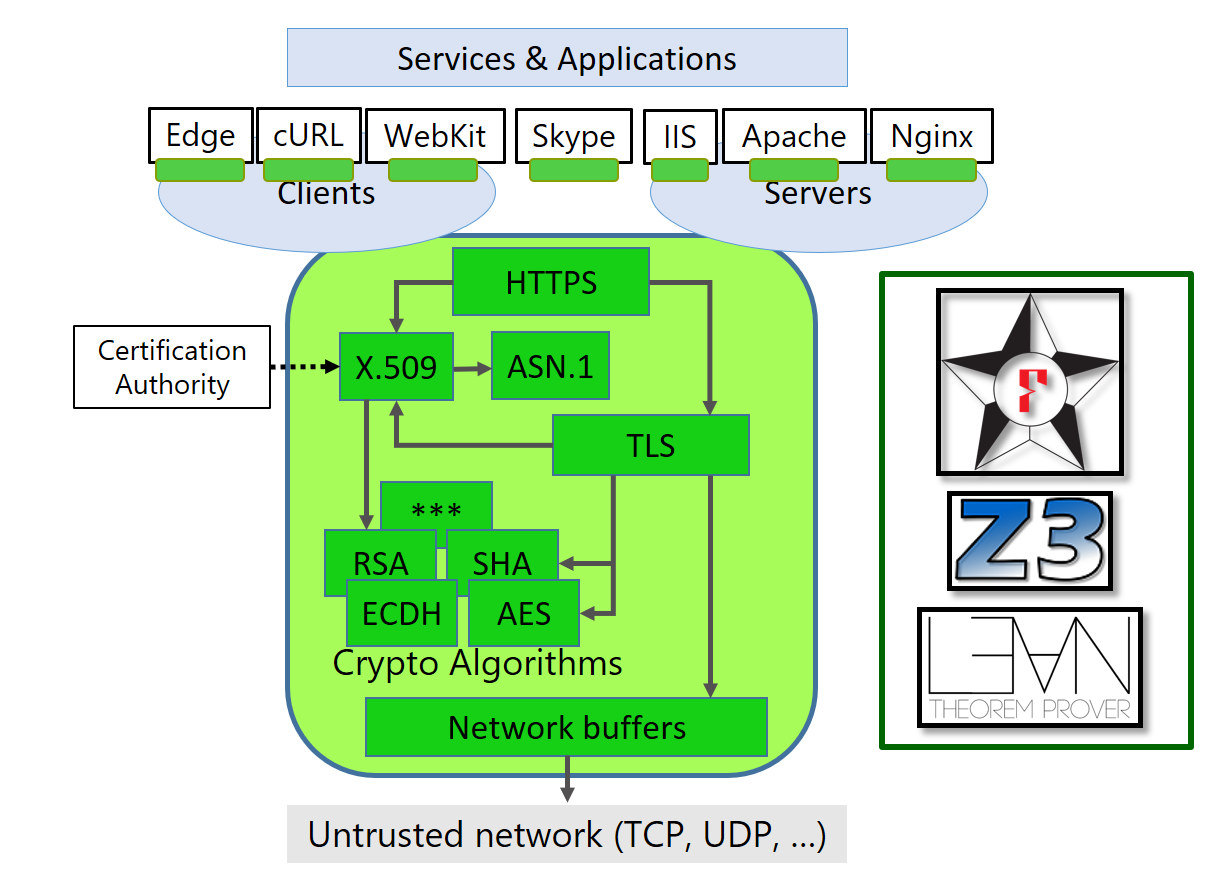
\includegraphics[scale=0.2]{SecureHTTPS.png}
  \end{center}

\end{frame}

\begin{frame}
  \frametitle{F*}

  \Fstar is an \textsf{ML}-style general-purpose functional
  programming language with effects aimed at program verification.

  \bigskip

  It was designed and developed at the joint Microsoft Research-Inria
  Center.

  \bigskip

  \Fstar programs can be extracted to efficient \OCaml, \Fsharp, or
  \Clang code. The \Fstar typechecker aims at proving that programs
  meet their specifications using a combination of \textbf{SMT
    solving} and interactive proofs.

  \bigskip

  Like \Coq, \Fstar can also be helped with intermediate lemmas and
  tactics when it cannot prove automatically the properties of the
  code.

  \bigskip

  There is an online tutorial
  \small\url{https://www.fstar-lang.org/tutorial/}
\end{frame}

%% \begin{frame}
%%   \frametitle{F*}

%%   \begin{center}
%%     \includegraphics[scale=0.12]{InsecureHTTPS.eps}
%%     \includegraphics[scale=0.132]{SecureHTTPS.eps}
%%   \end{center}
%% \end{frame}

\begin{frame}[fragile]
  \frametitle{F*}
   Here is the factorial function in \Fstar:
\begin{alltt}
\small
\textbf{val} fact: n:int\{n \(\geqslant\) 0\} \(\rightarrow\) Tot int

\textbf{let rec} fact n =
  \textbf{match} n \textbf{with}
    0 \(\rightarrow\) 1
  | \_ \(\rightarrow\) n * fact (n-1)
\end{alltt}

The annotation `\texttt{\small n:int\{n \(\geqslant\) 0\}
  \(\rightarrow\) Tot int}' is requesting the \Fstar compiler to prove
that the factorial function terminates (\texttt{\small Tot}) and
returns a positive integer (\texttt{\small \{n \(\geqslant\) 0\}})
when given as input a positive integer.

\end{frame}


\begin{frame}
  \frametitle{F*}

  \Fstar proves the function terminates using \textbf{well-founded
    recursion}.

  \bigskip

  If the positivity constraint in the input \texttt{\small n:int\{n
    \(\geqslant\) 0\}} is removed, the typechecker of \Fstar informs
  that it cannot prove the property.

  \bigskip

  Indeed, if \(n < 0\), the function does not terminate and a stack
  overflow occurs.

\end{frame}


\begin{frame}
  \frametitle{The Intel Pentium bug}

  \begin{center}
    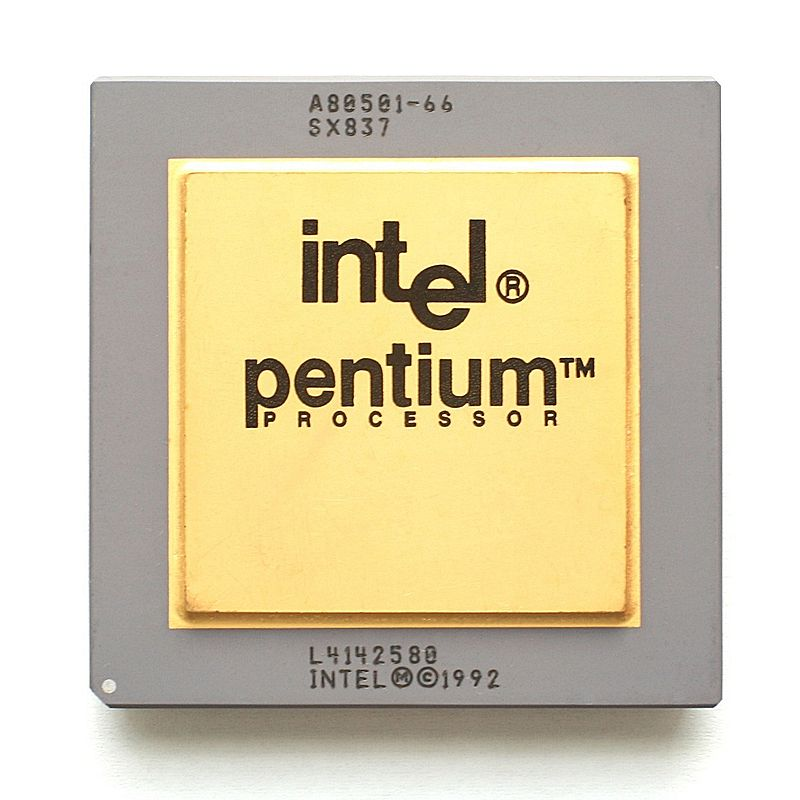
\includegraphics[scale=0.2]{Intel_Pentium_A80501.png}
  \end{center}

  \centerline{CPU Intel Pentium, 66 MHz. Credit: Konstantin Lanzet, CC
    BY-SA 3.0}
\end{frame}

\begin{frame}
  \frametitle{The Intel Pentium bug}

  \begin{itemize}

    \item The floating-point unit (FPU) of some Pentium processors
      (Intel) contained an error when a certain kind of division was
      performed.

    \item The FPU is a numeric coprocessor, to which the main
      processor (CPU) delegates computations for a speed up (about
      10$\times$).

    \item The error was discovered in 1994 by Thomas Nicely, a
      professor of mathematics at Lynchburg College (USA), who was
      performing number theoretic calculations.

    \item The division \emph{`\(1/824633702441.0\) is calculated
      incorrectly (all digits beyond the eighth significant digit are
      in error).' -- Thomas Nicely.}

    \item Intel had to recall all faulty units, incurring a large
      cost, but also a very bad press (CNN) in what was at the time a
      competitive market.

  \end{itemize}

\end{frame}

\begin{frame}
  \frametitle{The Intel Pentium bug}

  \begin{itemize}

    \item That bug is known as the `Intel Pentium FDIV bug', after
      the instruction for floating-point division.

    \item Intel reacted by investing in formal methods for the design
      of its chips.

    \item For example, John Harrison (Intel) has formally verified the
      correctness (of rounding) of various floating\hyp{}point
      algorithms using the \textbf{HOL Light prover} (a cousin of
      \Coq, also written in \OCaml).

    \item Also, various mathematical theorems in elementary number
      theory and real analysis were proved within the same framework.

    \item Intel combined theorem proving with a more automated
      approach when the state space is finite and small enough:
      \textbf{model checking}.

  \end{itemize}

\end{frame}

\begin{frame}
  \frametitle{Model checking}

  \textbf{Model checking} was invented in the 80s to check the
  properties of concurrent systems.  (Clarke, Emerson, and Sifakis
  shared the 2007 Turing Award for their work.)

  \bigskip

  Model checking reasons on the \textbf{states of a program}.

  \bigskip

  It requires a way to define
  \begin{itemize}

    \item all possible states of a program, including those that
      should not be reached, and

    \item the execution of a program as the \textbf{transition} from
      one state to another (\textbf{traces}).

  \end{itemize}

  \medskip

  There is usually a very large, but \textbf{finite number of states}.

\end{frame}


\begin{frame}
  \frametitle{Model checking}

  \textbf{Temporal logic} is used to express properties of states
  \begin{itemize}

    \item \textbf{Safety}: a given (`bad') state can never be
      reached

    \item \textbf{Liveness}: a given (`good') state will eventually
      be reached

    \item \textbf{Reachability}: a given (`good') state can be
      reached.

  \end{itemize}

  \medskip

  States and sets of states are usually defined with \textbf{logical
    formulas}.

  \bigskip

  \textbf{SMT solvers} are often used to find a trace that leads to an
  undesirable state or prove the state is unreachable by exhausting
  all traces.

\end{frame}


\begin{frame}
  \frametitle{The takeaway}

  \begin{itemize}

    \item Bugs are everywhere and can be very costly.

    \item The \textbf{B method} helps manually narrowing the gap
      between specification and concrete implementation.

    \item \textbf{Abstract interpretation} runs an approximation of a
      program on an approximation of all possible inputs.

    \item Astrée, PolySpace and Frama-C are abstract interpreters
      written in \OCaml, used in the aerospace industry.

    \item \Coq is a \textbf{proof assistant} used to check
      mathematical theorems.

    \item \Coq is also used to write \textbf{certified compilers}.

  \end{itemize}

\end{frame}

\begin{frame}
  \frametitle{The takeaway}

  \begin{itemize}

    \item \Fstar enables proving properties of functions using
      \textbf{type annotations}.

    \item \Fstar automatically proves the termination of recursive
      functions using \textbf{well-founded recursion}, but does not
      always succeed.

    \item \Fstar has been used to write efficient certified
      cryptographic libraries.

    \item \textbf{Model checking} is a technique to analyse all
      possible states of a program and prove that some (bad) states
      are unreacheable.

    \item States and sets of states are defined with \textbf{logical
      formulas}.

    \item \textbf{SMT solvers} are used to find a trace reaching
      undesired states, or prove the absence of such a trace.

%    \item CubicleW is a model checker written in OCaml, used by Intel
%      to check processor pipeline reordering

  \end{itemize}

\end{frame}


\end{document}
